\documentclass[12pt,a4paper]{article}
\usepackage{algorithm, algpseudocode, amsmath, amssymb, amsthm, csquotes, empheq, geometry, graphicx, hyperref, listings, multirow, siunitx, subcaption, upgreek}
\usepackage[italicdiff]{physics}
\usepackage[section]{placeins}
\usepackage[justification=centering]{caption}

\title{Computational Physics\\Problem Set 7}
\author{Saleh Shamloo Ahmadi\\Student Number: 98100872}
\date{November 8, 2021}

\hypersetup{colorlinks=true, urlcolor=cyan}
\newcommand{\fig}{../fig}
\newcommand{\ddfrac}[2]{{\displaystyle\frac{\displaystyle #1}{\displaystyle #2}}}
\newcommand{\multlinecell}[1]{\begin{tabular}[c]{@{}c@{}}#1\end{tabular}}

\begin{document}
	\maketitle
    \section{Monte Carlo Integration}
    \subsection[pi/2 * erf(2): Uniform Sampling vs. Importance Sampling]
    {Uniform Sampling vs. Importance Sampling:\\$\frac{\sqrt{\pi}}{2}\erf(2)=\int_0^2 e^{-x^2} \dd{x}$}
    \begin{table}[hbt!]
        \centering
        \caption{The exact value of the integral $\frac{\sqrt{\pi}}{2}\erf(2)=\int_0^2 e^{-x^2} \dd{x}$
            up to the 6th decimal is $0.882081$. The runtimes are from an AMD Ryzen 7 5800H @3.2GHz (up to 4.4GHz)}
        \begin{tabular}{|c|c|c|c|c|}
            \hline
            \multirow{2}{*}{\multlinecell{Number\\of\\Samples}}
            & \multicolumn{2}{|c|}{Calculated Integral} & \multicolumn{2}{|c|}{Runtime} \\
            \cline{2-5}
            & \multlinecell{Uniform\\Sampling} & \multlinecell{Importance\\Sampling}
            & \multlinecell{Uniform\\Sampling} & \multlinecell{Importance\\Sampling} \\
            \hline
            $10$ & $0.460596$ & $0.93583$ & $\SI{0.891513}{\micro\second}$ & $\SI{3.74894}{\micro\second}$ \\
            $100$ & $0.921345$ & $0.903689$ & $\SI{1.6772}{\micro\second}$ & $\SI{21.2343}{\micro\second}$ \\
            $1000$ & $0.899169$ & $0.882798$ & $\SI{8.6187}{\micro\second}$ & $\SI{183.041}{\micro\second}$ \\
            $10000$ & $0.889229$ & $0.880103$ & $\SI{79.3509}{\micro\second}$ & $\SI{1.82276}{\milli\second}$ \\
            $100000$ & $0.880586$ & $0.881593$ & $\SI{844.887}{\micro\second}$ & $\SI{18.7801}{\milli\second}$ \\
            $1000000$ & $0.880835$ & $0.882562$ & $\SI{9.04039}{\milli\second}$ & $\SI{178.5040}{\milli\second}$ \\
            $10^7$ & $0.882187$ & $0.88204$ & $\SI{93.6652}{\milli\second}$ & $\SI{2.51925}{\second}$ \\
            $10^8$ & $0.882014$ & $0.882084$ & $\SI{0.919785}{\second}$ & $\SI{23.3132}{\second}$ \\
            \hline
        \end{tabular}
    \end{table}
    \begin{table}[hbt!]
        \centering
        \caption{Errors of each method. The \enquote{actual} error is the deviation of the calculation from
            $\frac{\pi}{2}\erf(2)$.}
        \begin{tabular}{|c|c|c|c|c|}
            \hline
            \multirow{2}{*}{\multlinecell{Number\\of\\Samples}}
            & \multicolumn{2}{|c|}{Calculated Standard Error} & \multicolumn{2}{|c|}{Actual Error} \\
            \cline{2-5}
            & \multlinecell{Uniform\\Sampling} & \multlinecell{Importance\\Sampling}
            & \multlinecell{Uniform\\Sampling} & \multlinecell{Importance\\Sampling} \\
            \hline
            $10$ & $0.211308$ & $0.094789$ & $0.421485$ & $0.0537491$ \\
            $100$ & $0.0699633$ & $0.0242373$ & $0.0392635$ & $0.021608$ \\
            $1000$ & $0.0220645$ & $0.00838951$ & $0.0170874$ & $0.000716757$ \\
            $10000$ & $0.00685873$ & $0.0026753$ & $0.00714762$ & $0.00197877$ \\
            $100000$ & $0.00217824$ & $0.000843176$ & $0.00149538$ & $0.000488134$ \\
            $1000000$ & $0.000688905$ & $0.000265692$ & $0.00124646$ & $0.000480197$ \\
            $10^7$ & $0.000217995$ & $\num{8.41355e-5}$ & $0.000106063$ & $\num{4.187e-5}$ \\
            $10^8$ & $\num{6.89327e-5}$ & $\num{2.66006e-5}$ & $\num{6.72089e-5}$ & $\num{2.30387e-6}$ \\
            \hline
        \end{tabular}
    \end{table}
    \begin{figure}[htb!]
        \centering
        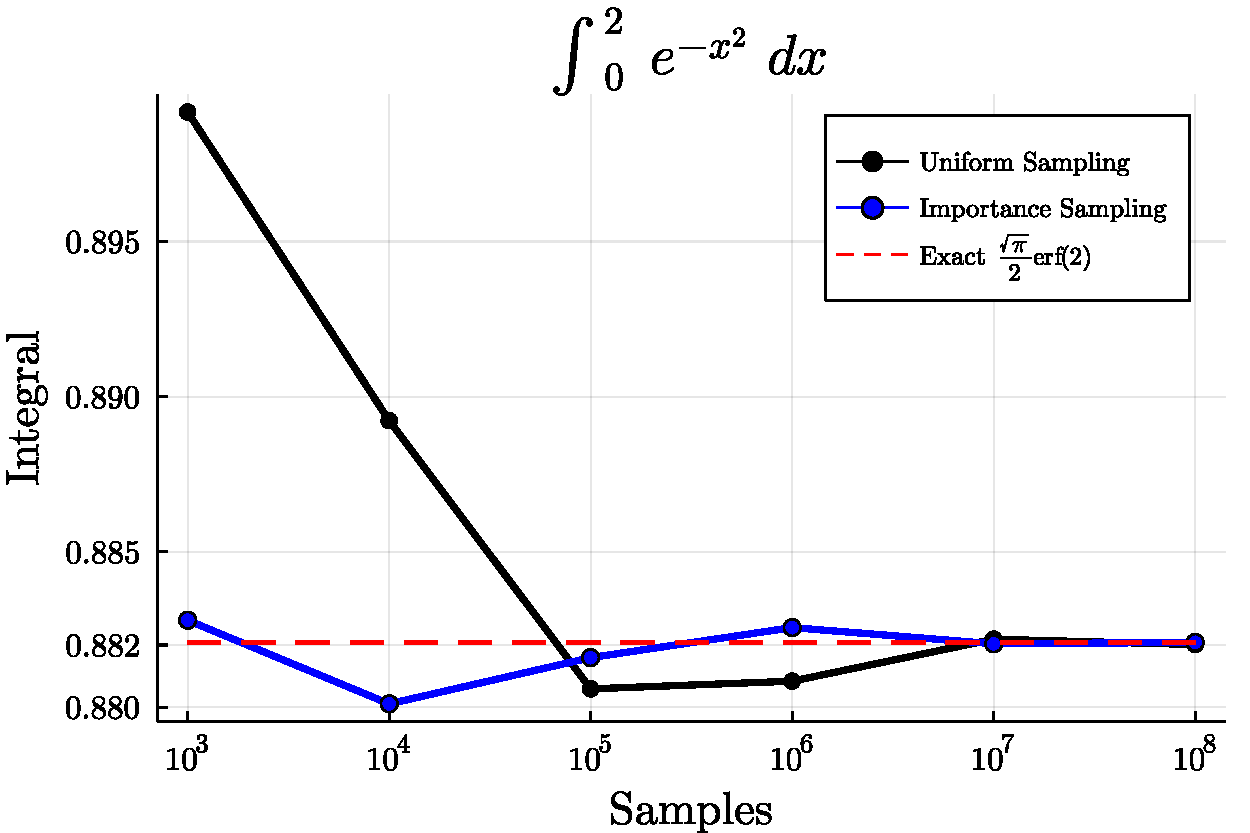
\includegraphics[width=\linewidth]{\fig/montecarlo-erf2-value}
    \end{figure}
    \begin{figure}[htb!]
        \centering
        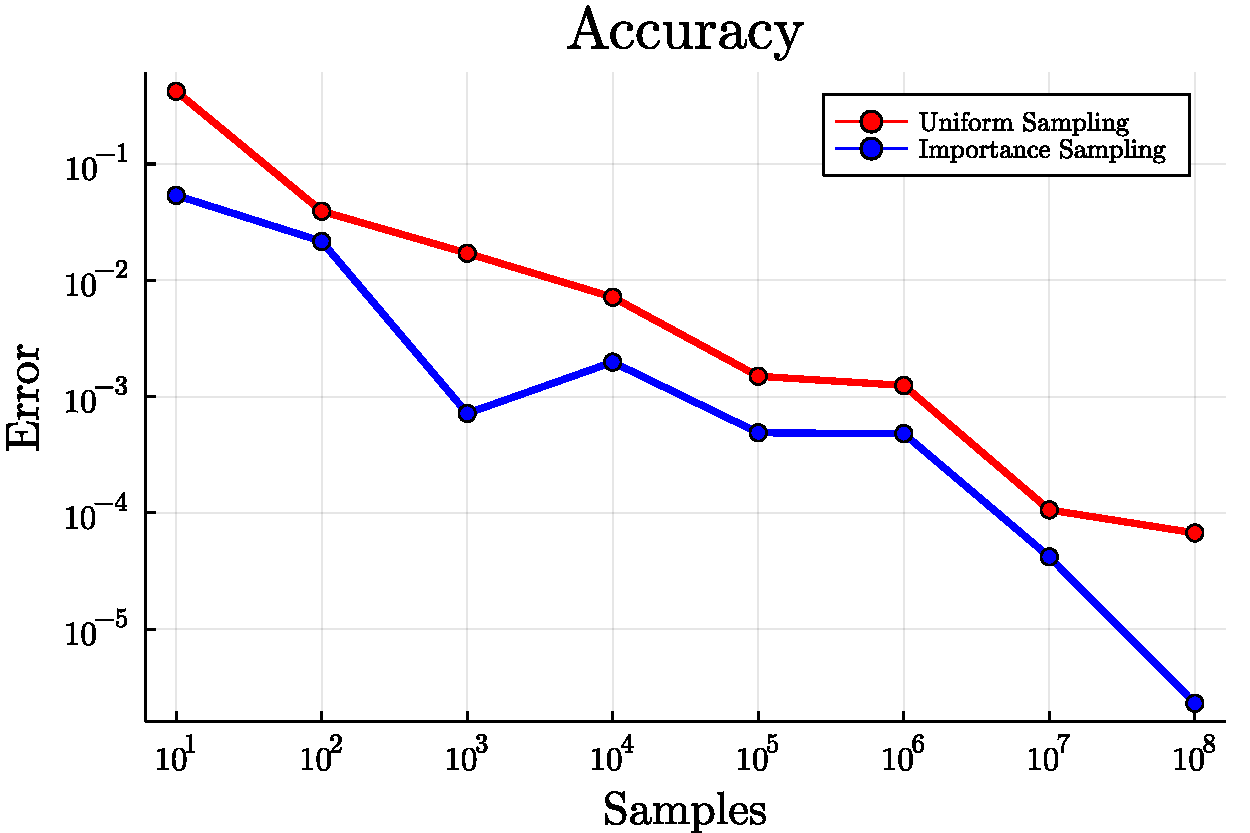
\includegraphics[width=\linewidth]{\fig/montecarlo-erf2-error}
    \end{figure}
    \begin{figure}[htb!]
        \centering
        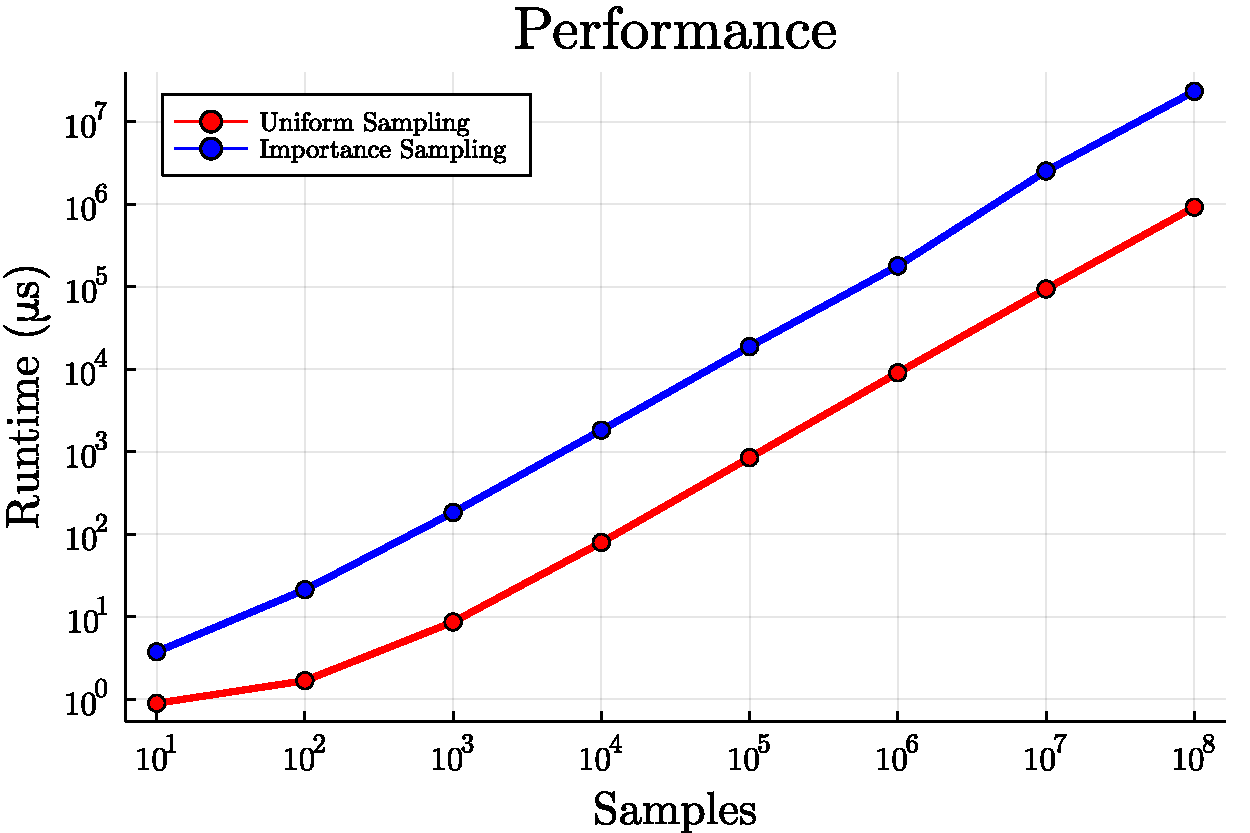
\includegraphics[width=\linewidth]{\fig/montecarlo-erf2-time}
    \end{figure}
    \FloatBarrier
    \subsection{Center of Mass of Sphere with Linearly Increasing Density in One Direction}
    A sphere with radius $R$ has a density that linearly increases in the $z$ direction, such that the density at $z=2R$
    is twice the density at $z=0$. To calculate the position of the center of mass, we must evaluate the integral
    \begin{equation}
        \vb{r}_{cm} = \frac{\int_{\text{sphere}}\rho(\vb{r})\vb{r}\dd{V}}{\int_{\text{sphere}}\rho(\vb{r})\dd{V}}.
    \end{equation}
    Since the sphere is symmetric in the $x$ and $y$ directions, the center of mass is at $x=0$ and $y=0$. It remains to
    find the $z$ position of the center of mass. In polar coordinates
    \begin{gather}
        \rho(z=2R) = 2\rho(z=0) \implies \rho(r=R, \theta=0) = 2\rho(r=R, \theta=\pi) \\
        \xRightarrow{\rho(z) is linear} \rho(r, \theta) = \rho_0\qty(3+\frac{r}{R}\cos{\theta}) \implies \\
        z_{cm} = \ddfrac{\int_{\text{sphere}}z\rho\dd{V}}{\int_{\text{sphere}}\rho\dd{V}} =
        \ddfrac{\int_0^R\int_0^\pi\int_0^{2\pi} \rho_0\qty(3+\frac{r}{R}\cos{\theta})r^3\sin{\theta}\cos{\theta}
        \dd{\varphi}\dd{\theta}\dd{r}}{\int_0^R\int_0^\pi\int_0^{2\pi} \rho_0\qty(3+\frac{r}{R}\cos{\theta})r^2
        \sin{\theta}\dd{\varphi}\dd{\theta}\dd{r}} \\
        z_{cm} = \ddfrac{\int_0^R\int_0^\pi \qty(3+\frac{r}{R}\cos{\theta})r^3\sin{\theta}\cos{\theta}
        \dd{\theta}\dd{r}}{\int_0^R\int_0^\pi \qty(3+\frac{r}{R}\cos{\theta})r^2\sin{\theta}
        \dd{\theta}\dd{r}} \label{eq:multi}
    \end{gather}
    We can use the Monte Carlo integration method to calculate \eqref{eq:multi} and find the center of mass.
    These integrals can also be calculated analytically to check the accuracy of the numerical results:
    \begin{align}
        z_{cm} &= \ddfrac{R^4 \int_0^\pi \qty(\frac{3}{4}+\frac{\cos{\theta}}{5})\sin{\theta}\cos{\theta}\dd{\theta}}
        {R^3 \int_0^\pi \qty(1+\frac{\cos{\theta}}{4})\sin{\theta}\dd{\theta}} \\
        &= \ddfrac{\frac{3}{8}\int_0^\pi\sin(2\theta)\dd{\theta} + \frac{1}{5}\int_{-1}^{+1}\cos^2{\theta}
        \dd{(\cos{\theta})}} {\int_0^\pi\qty(\sin{\theta} + \frac{\sin(2\theta)}{2})\dd{\theta}}R \\
        &= \frac{-\frac{3}{16}\eval{\cos(2\theta)}_0^\pi + \eval{\frac{x^3}{15}}_{-1}^{+1}}
        {-\eval{\cos{\theta}}_0^\pi - \eval{\frac{\cos(2\theta)}{4}}_0^\pi}
    \end{align}
    \begin{empheq}[box=\fbox]{equation}
        z_{cm} = \frac{R}{15}
    \end{empheq}
    Numerically evaluating the two integrals in \eqref{eq:multi} by the Monte Carlo Integration method,
    uniformly sampling 40 million points, we get
    \begin{equation}
        z_{cm} = (0.06667 \pm 0.00009) R,
    \end{equation}
    which is exactly equal to $R/15$ up to the 5th decimal place.
    \section{Metropolis Algorithm}
    \begin{table}[hbt!]
        \centering
        \caption{For $10^8$ samples}
        \begin{tabular}{|c|c|c|}
            \hline
            Step Size $Delta$ & Acceptance Rate $a_r$ & Correlation Length $\xi$ \\
            \hline
            15.8846 & 0.1004 & $7.23 \pm 0.03$ \\
            7.969 & 0.19996 & $3.53 \pm 0.03$ \\
            5.3048 & 0.300005 & $2.3 \pm 0.03$ \\
            3.888 & 0.4003 & $1.84 \pm 0.01$ \\
            2.9486 & 0.4991 & $2.06 \pm 0.02$ \\
            2.2094 & 0.5992 & $2.72 \pm 0.02$ \\
            1.578 & 0.7007 & $4.11 \pm 0.02$ \\
            1.0236 & 0.8002 & $7.89 \pm 0.02$ \\
            0.5 & 0.9008 & $27.76 \pm 0.01$ \\
            \hline
        \end{tabular}
    \end{table}
    \begin{figure}[htb!]
        \centering
        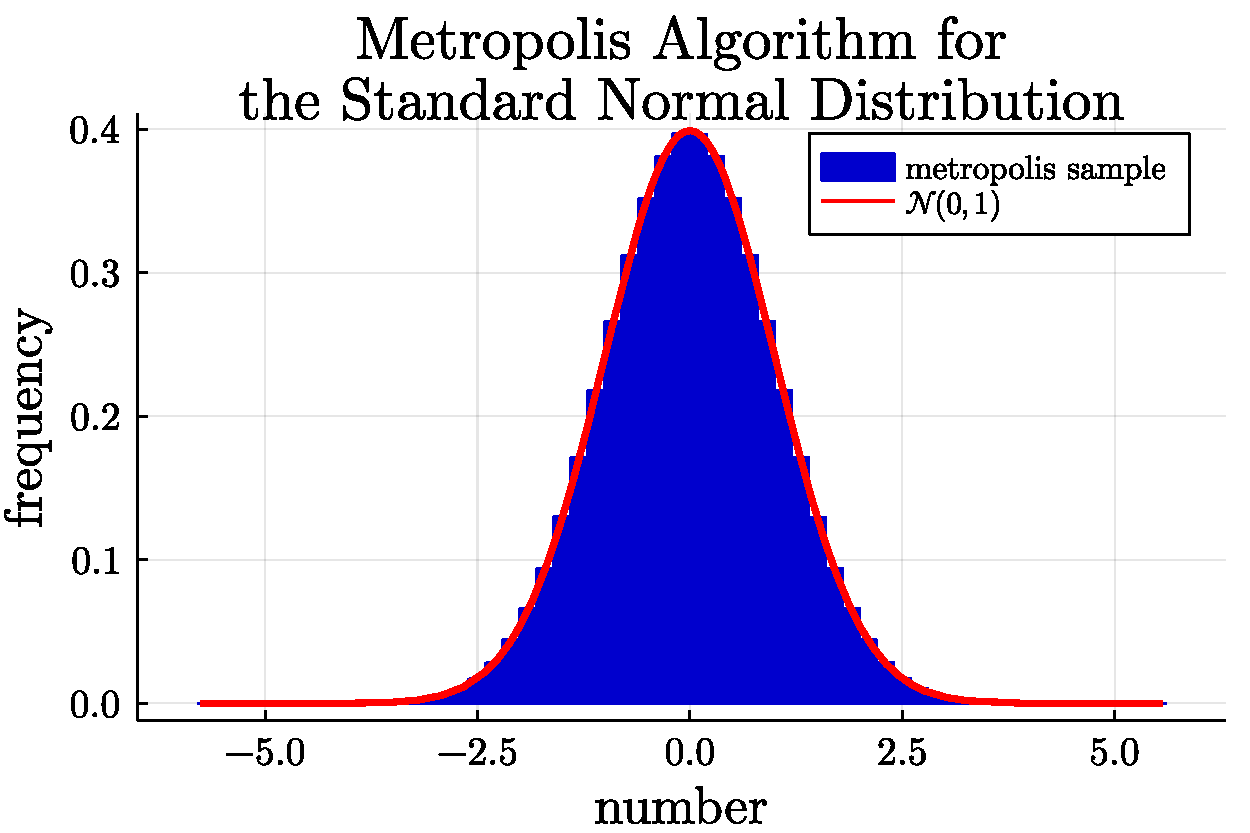
\includegraphics[width=0.65\linewidth]{\fig/metropolis-hist}
        \caption{For $10^8$ samples, step size 3 and acceptance rate 0.49}
    \end{figure}
    \begin{figure}[htb!]
        \centering
        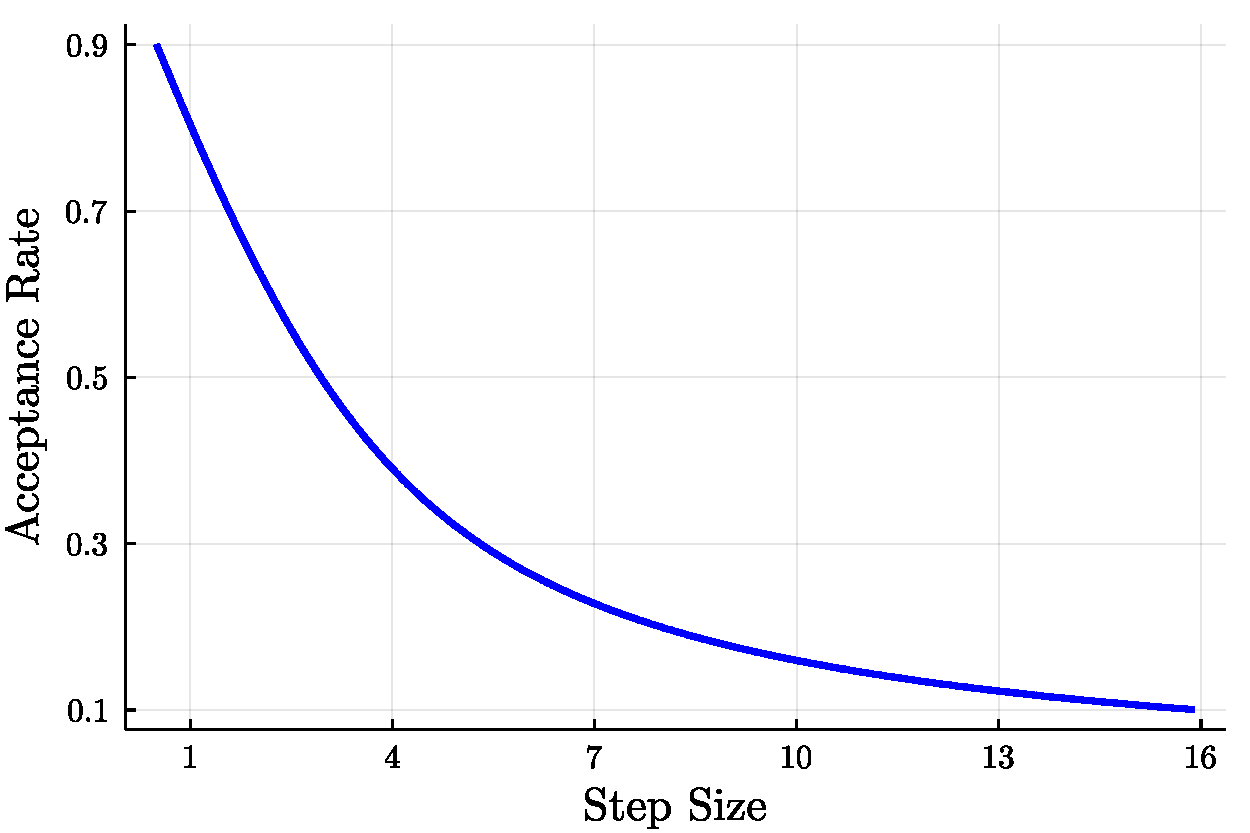
\includegraphics[width=\linewidth]{\fig/metropolis-acceptance}
    \end{figure}
    \begin{figure}[htb!]
        \centering
        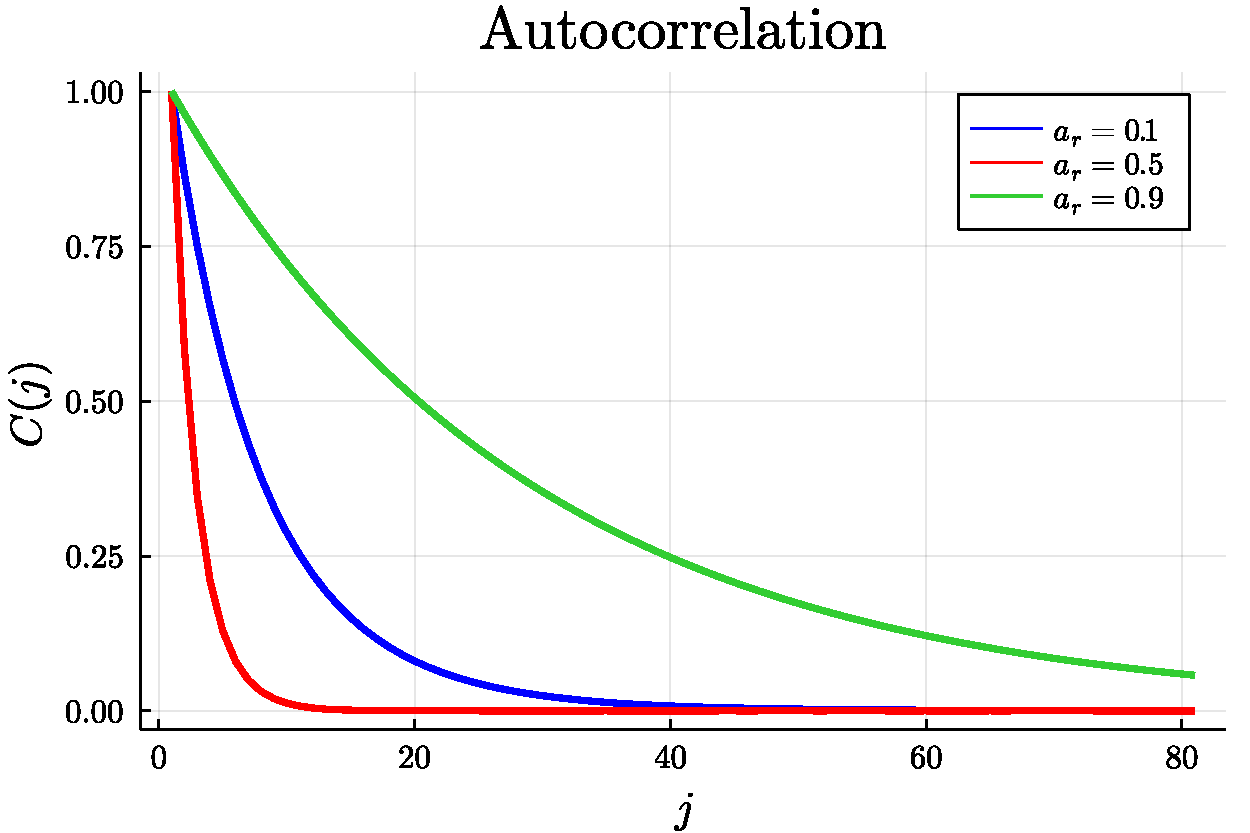
\includegraphics[width=\linewidth]{\fig/metropolis-autocor}
    \end{figure}
    \begin{figure}[htb!]
        \centering
        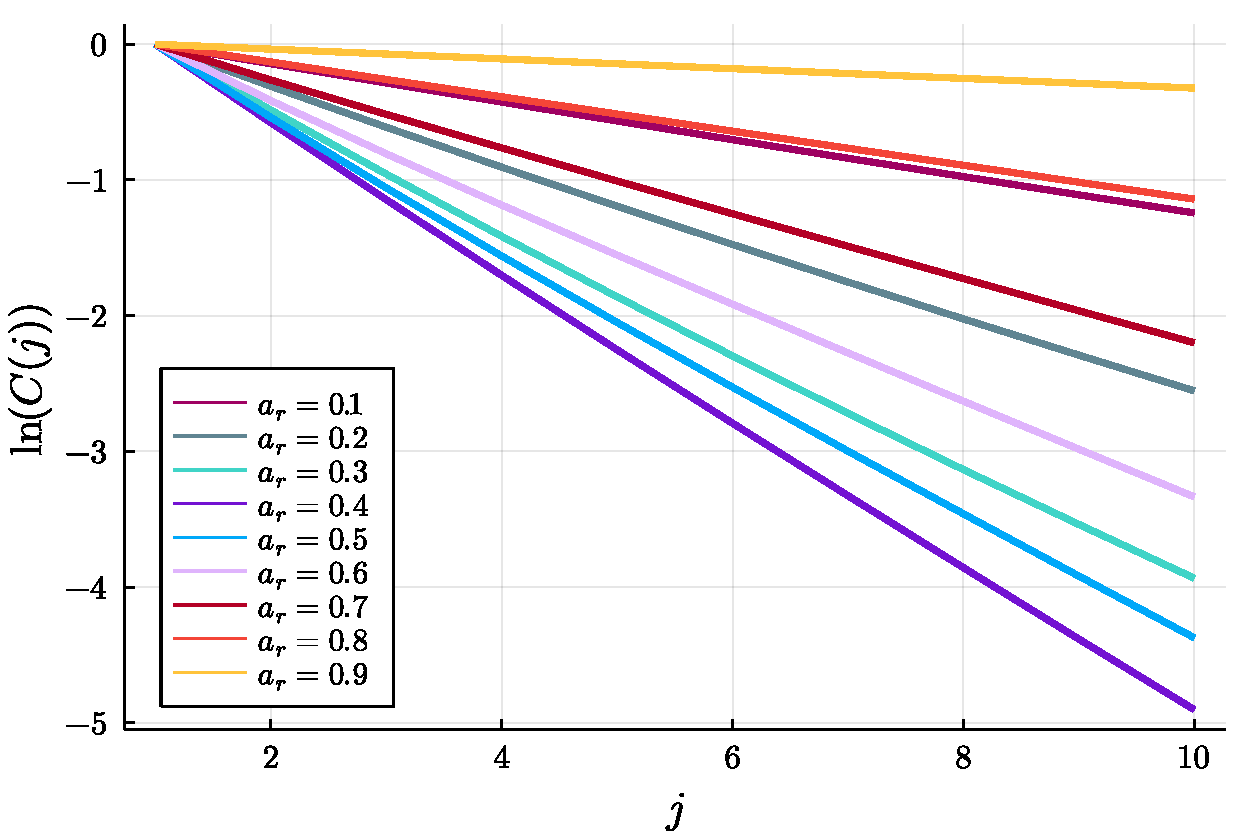
\includegraphics[width=\linewidth]{\fig/metropolis-autocor-log}
    \end{figure}
    \begin{figure}[htb!]
        \centering
        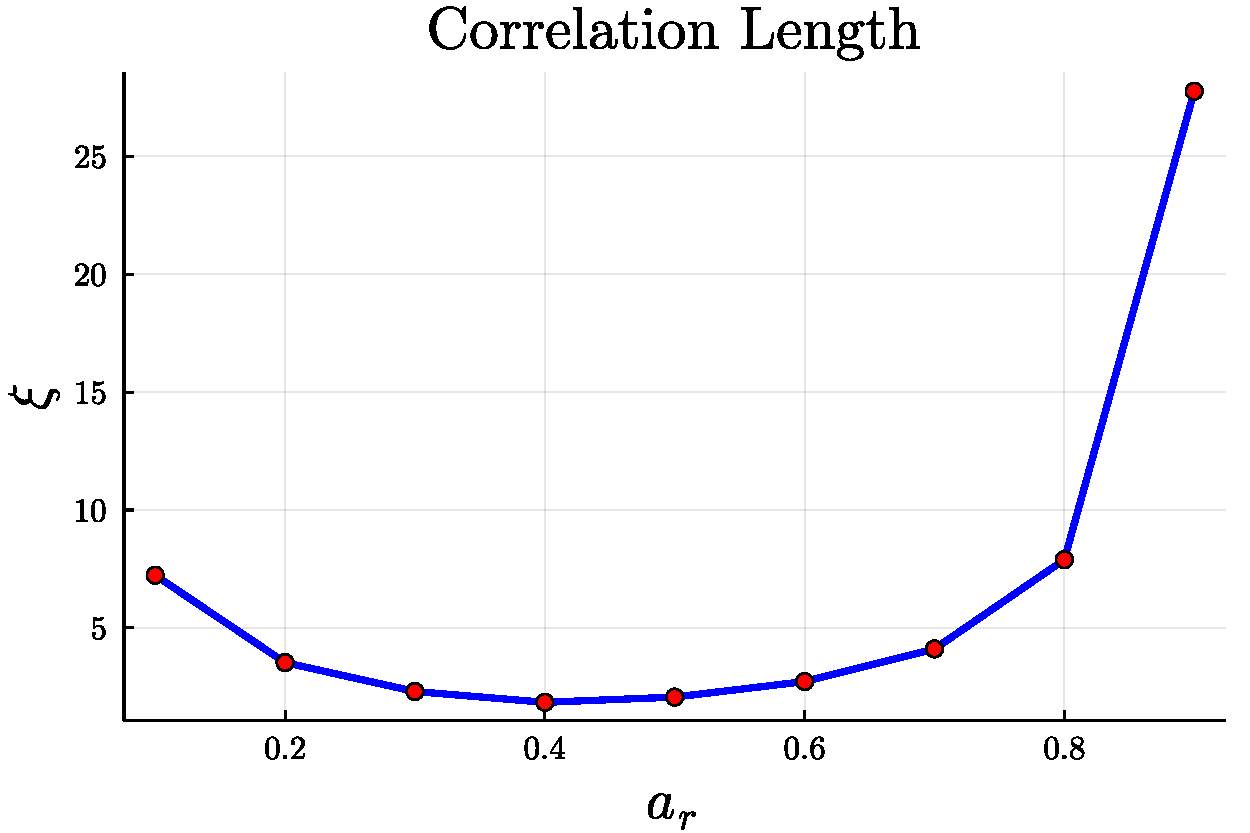
\includegraphics[width=\linewidth]{\fig/metropolis-corlen}
    \end{figure}
\end{document}
